% !TeX root = Trafficsimulation_Documentation.tex

\chapter{Implementierung}
\label{Implementierung}

In diesem Kapitel werden die Implementierungen der einzelnen Komponenten sowie deren Schnittstellen zu anderen Komponenten dokumentiert.

\thispagestyle{standard}
\pagestyle{standard}

\section{Erstellung der Welt}
\label{Erstellung_der_Welt}


In der Verkehrssimulation können beliebige Strassennetze gebaut werden. Dazu stehen Verschiedene vordefinierte Elemente zur Verfügung. Dazu zählen T- und X-Kreuzungen, Kurven, Geraden und Spawn Flächen. In den Elementen sind alle benötigten Komponenten und Skripte vorhanden und diese können einfach mit Drag and Drop in die Simulation gezogen und platziert werden. Es ist nur darauf zu achten, dass
alle Strassenelemente welche zusammengehören, also zwei Kreuzungen verbinden in einem übergeordneten GameObject zusammengefasst werden. Ein Beispiel ist in Abbildung \ref{img:streetbbuild} dargestellt.

\begin{figure}[H]
\begin{center}
	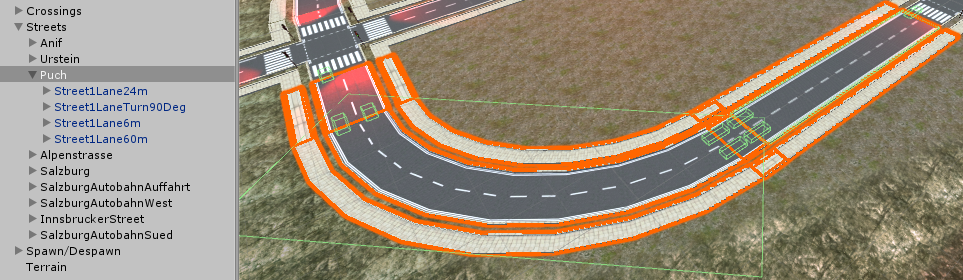
\includegraphics[width=1\textwidth]{BilderAllgemein/streetImpl.PNG}
\end{center}
	\caption{Aufbau des Strassennetzes}
	\label{img:streetbbuild}
\end{figure}

Im rechten Teil der Abbildung sind die Strassenelemente abgebildet. In diesem Beispiel lautet der Übergeordnete Strassenname \grqq Puch\grqq. In Diesem GameObject \grqq Puch\grqq{} sind alle Teilstücke der Strasse vorhanden. Diese müssen dabei in auf- oder absteigender Reihenfolge angeordnet sein.

Kreuzungen können auch beliebig mit Drag and Drop eingefügt werden. Dabei müssen die Strassen den Kreuzungen bekannt gegeben werden. Beim Klick auf das jeweilige erzeugte Element kann rechts in den Skript Einstellungen kann ausgewählt werden, ob die Kreuzung geregelt oder ungeregelt sein soll.
Weiters müssen die angeschlossenen Strassen eingefügt werden. Ein Beispiel ist in Abbildung \ref{img:crossbuild} dargestellt. Es wurde das vorher erstellte Strassenelement angeschlossen 

\begin{figure}[H]
\begin{center}
	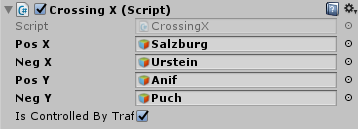
\includegraphics[width=0.65\textwidth]{BilderAllgemein/crossingImpl.PNG}
\end{center}
	\caption{Einstellungen für eine Kreuzung}
	\label{img:crossbuild}
\end{figure}

Die Richtungen (Pos X, Neg Y, etc.) sind an das Koordinaten System des Kreuzungselementes angelehnt. Bei einem Klick auf die Kreuzung erscheint das Koordinaten System. Daran kann erkannt werden, an welcher Stelle die jeweilige Strasse eingetragen werden muss.

\section{Fahrzeugsteuerung}
\label{Fahrzeugsteuerung}

Die Fahrzeugsteuerung ist zuständig für das Folgen der Strasse und das richtige Abbiegen des Autos. Diese Funktionen werden im Skript 'FollowWay.cs' des Fahrzeugs verwirklicht.

\subsection{Folgen der Strasse}
Wie in Kapitel \ref{sub:street} beschrieben befinden sich auf jeder Strasse Wegpunkte. Fährt ein Fahrzeug auf eine neue Strasse bekommt es von der Kreuzung die Richtung und das GameObject der Strasse übergeben. Das Fahrzeug bewegt sich dabei von Wegpunkt zu Wegpunkt mithilfe des in \ref{lst:FollowWay} dargestellten Codes.

\begin{lstlisting}[caption={Transformation der Fahrzeuge},label={lst:FollowWay}]
 dir = targetPathNode.position;
 dir = dir - this.transform.localPosition; 	//Berechnung der Richtung

 float distThisFrame = speed * Time.deltaTime;		//Berechnung der zu bewegenden Distanz

 transform.Translate(dir.normalized * distThisFrame, Space.World);		//Verschieben des Objekts
 Quaternion targetRotation = Quaternion.LookRotation(dir);			
 this.transform.rotation = Quaternion.Lerp(this.transform.rotation, targetRotation, Time.deltaTime * rotationSpeed);	//Rotieren des Objekts
\end{lstlisting}

Die Berechnung der Verschiebung erfolgt aufgrund der aktuellen Position des Fahrzeugs und der Position des Wegpunktes. Dabei wird auch die aktuelle Geschwindigkeit des Fahrzeuges einbezogen.

Das Bewegen des Fahrzeugs findet in der 'update()' Methode statt. Diese wird regelmäßig von der Game Engine aufgerufen. Da die Abstände dieses Aufrufs variieren können wird auch die Zeit des letzten Aufrufs in die Berechnung einbezogen.

Befindet sich das Fahrzeug auf einem der Wegpunkte wird in der Methode 'getNextStreetPart()' der nächste Wegpunkt bestimmt. Es können dabei drei Fälle auftreten. Befindet sich auf der aktuellen 
Strasse noch ein Wegpunkt wird dieser angefahren. Befindet sich auf diesem Strassenelement kein Wegpunkt mehr, wird das nächste Strassenelement aus der von der Kreuzung erhaltenen Strasse gewählt und aufgrund der Richtung (Pos od. Neg) wird auf dem neuen Strassenelement der nächste Wegpunkt gewählt.

Ist kein neues Strassenelement vorhanden, fährt das Fahrzeug auf eine Kreuzung zu und es bekommt die nächsten Wegpunkte bei der Kollision mit den Collidern der Kreuzung. 

\subsection{Abbiegen bei Kreuzungen}

Fährt ein Fahrzeug auf eine Kreuzung zu, kollidiert es mit dem an der Kreuzungs Einfahrt befindlichen Collider. Dadurch wird der in Listing \ref{lst:decideWay} dargestellte Code ausgeführt.

\begin{lstlisting}[caption={Abbiegeentscheidung auf einer Kreuzung},label={lst:decideWay}]
public void decideWay(CrossingColliderX collider)
    {
        if(!isNewStreet)
        {
            System.Random random = new System.Random();
            int randomNumber = random.Next(0, 3);
            nextCrossingColliderT = null;
            nextCrossingColliderX = collider;
            collider.setDirection(randomNumber, this);
        }

    }
\end{lstlisting}

Zuerst entscheidet das Fahrzeug mithilfe einer Zufallszahl in welche Richtung das Fahrzeug fahren soll. Danach wird eine Methode des Kreuzungs Skripts aufgerufen. Als Parameter werdenr Information für die nächste Richtung (die vorher erstellte ZZ) und das eigene Objekt für ein Callback übergeben.
Im Skript der Kreuzung wird aufgrund dieser Informationen durch den Aufruf einer Methode des Fahrzeugs die nächsten Wegpunkte auf der Kreuzung und der nächste Strassenabschnitt weitergeben.
% 

\section{Erkennen und Reagieren auf Ampeln}
\label{Erkennen_und_Reagieren_auf_Ampeln}

Das Event 'OnTriggerEnter' wird beim kollidieren mit Collidern generiert. In diesem Event, welches im 'FollowWay.cs' Skript implementiert wurde, wird überprüft, zu wem der kollidierte Collider gehört. Wird hierbei ein Ampelcollider erkannt, so wird dieser zwischengespeichert, sonst werden noch die anderen Collider auf der Kreuzung erkannt und es kommt zum Fehlverhalten im Fahrzeug. Die Bezeichnungen 'PosX', 'NegX', 'PosY' und 'NegY' beschreiben hierbei die Ampelpositionen.

\begin{lstlisting}[caption={Erstes erkennen einer Ampel},label={lst:ampel_erkennen}]
void OnTriggerEnter(Collider collider)
{
	GameObject itself = gameObject;
	GameObject colliededObject = collider.gameObject;

	float distance = getDistance(itself, colliededObject);
	if((colliededObject.name.Equals("PosX") ||
		colliededObject.name.Equals("NegX") ||
		colliededObject.name.Equals("PosY") ||
		colliededObject.name.Equals("NegY")) && (firstCollider == null))
	{
		//Here the car collided with a crossing collider
		crossingCurrent = collider.transform.parent.gameObject.transform.parent.gameObject; //The current crossing?!
		firstCollider = colliededObject;
	}
}
\end{lstlisting}

Nun wird das Event 'OnTriggerStay' aufgerufen, da sich das Fahrzeug immer noch im Collider der Ampel befindet. In diesem Event wird zwischen den zwei verschiedenen Kreuzungstypen, T- und X-Kreuzung unterschieden. Von diesen Kreuzungen wird sich dann eine Referenz geholt und den aktuellen Status der Ampel abgefragt. Je nach Status der Ampel verhält sich das Fahrzeug anders. Diese Verhalten wird in der 'carDecisionOnCrossing' Funktion festgelegt. Folgende Ampelverhalten wurden festgelegt:

\begin{itemize}  
\item \textbf{Grün:} Beschleunigen
\item \textbf{Blinkend Grün:} Beschleunigen
\item \textbf{Gelb:} Bremsen
\item \textbf{Blinkend Gelb:} Geschwindigkeit beibehalten
\item \textbf{Rot Gelb:} Beschleunigen
\item \textbf{Rot:} Bremsen
\end{itemize}

\begin{lstlisting}[caption={Bestehende Kollision mit Ampelcollider},label={lst:ampel_decision}]
void OnTriggerStay(Collider collider)
{
	GameObject collidedObject = collider.gameObject;

	if(collidedObject.name.Equals("PosX") ||
	collidedObject.name.Equals("NegX") ||
	collidedObject.name.Equals("PosY") ||
	collidedObject.name.Equals("NegY"))
	{
		CrossingColliderT crossT = null;
		CrossingColliderX crossX = null;

		float distance = getDistance(gameObject, collidedObject);
		if(collidedObject == firstCollider)
		{
			crossT = collidedObject.GetComponentInParent<CrossingColliderT>();
			if(crossT == null)
			{
				crossX = collidedObject.GetComponentInParent<CrossingColliderX>();
				if(crossX == null)
				{
					return;
				}
				RemoteObject.Enum.TrafficLightsStatus trafficLightStatus = crossX.actLightState;
				carDecisionOnCrossing(trafficLightStatus, distance);
			}
			else
			{
				RemoteObject.Enum.TrafficLightsStatus trafficLightStatus = crossT.actLightState;
				carDecisionOnCrossing(trafficLightStatus, distance);
			}
		}
	}
}
\end{lstlisting}

Die an den Fahrzeugen sitzenden Collider werden in jedem Update Aufruf je nach Geschwindigkeit des Fahrzeuges vergrößert bzw. verkleinert, so kann auf Ampeln hingebremst werden und kein abruptes Stehenbleiben erzwungen werden.

\section{Fahrzeug Kollisionserkennung}
\label{Fahrzeug_Kollisionserkennung}

Jedes Fahrzeug implementiert das 'FollowWay.cs' Skript welches die komplette Logik über das Verkehrsverhalten besitzt. Innerhalb dieses Skripts wird in der Update-Methode, welche in jedem Frame pro Sekunde aufgerufen wird, überprüft, ob ein Raycast mit einem anderen Fahrzeug oder Hindernis kollidiert ist. Da dieser Raycast mehrere Objekte durchdringen kann, muss in einer Liste überprüft werden ob mit einem dieser Objekte kollidiert werden soll. Ist dies der Fall, so wird die Geschwindigkeit des Fahrzeugs verringert und der Raycast wird auf die Länge, welche der Geschwindigkeit des Fahrzeugs entspricht, gesetzt. Dazu wird die Distanz des zu kollidierenden Objekts und dem Fahrzeug ermittelt. Mit der Distanz wird das Fahrzeug dann entsprechend abgebremst und wenn nötig auch zum Stillstand gebracht. Um nicht in das vorherfahrende Objekt zu fahren, wird die Hälfte der Länge des Fahrzeugs noch von der Distanz abgezogen. Damit sich das Fahrzeug nicht selbst als kollidierendes Objekt erkennt, muss der Layer des Fahrzeugs für kurze Zeit geändert werden.

\begin{lstlisting}[caption={Erkennen von anderen Fahrzeugen und Hindernissen},label={lst:Hinderniss_erkennen}]
private void checkRaycast()
{
	// Save current object layer
	int oldLayer = gameObject.layer;
	//Change object layer to a layer it will be alone
	gameObject.layer = 12;
	int layerToIgnore = 1 << 12;
	layerToIgnore = ~layerToIgnore;

	RaycastHit[] hits;		
	hits = Physics.RaycastAll(transform.position, transform.forward, raycastSize, layerToIgnore);
	bool somethingInFront = false;
	for(int i = 0; i < hits.Length; i++)
	{
		RaycastHit hit = hits[i];
		GameObject collidedObject = hit.collider.gameObject;
		if(collidedObject.name.Equals("jeep(Clone)") || collidedObject.name.Equals("Rock(Clone)"))
		{
			float distance = getDistance(gameObject, collidedObject);
			if(gameObject.name.Equals("jeep(Clone)"))
			{
				distance = distance - (lengthCar / 2 + 1f);
			}
			else
			{
				distance = distance - (lengthTanker / 2 + 1f);
			}
			brakeWithDistance(distance);
			mayIdrive = false;
			somethingInFront = true;
		}
		if(somethingInFront == false)
		{
			mayIdrive = true;
		}
	}
	raycastSize = speed;
	if(raycastSize < 1)
	{
		raycastSize = 1;
	}
	// set the game object back to its original layer
	gameObject.layer = oldLayer;
}
\end{lstlisting}

\section{Ampelsteuerung}
\label{Ampelsteuerung}

Die Ampelsteuerung wurde als eigene Applikation entwickelt. Die Ampelsteuerung kann grundsätzlich unabhängig von der Unity-Spielwelt laufen, auch die Ampeln schalten dementsprechend autonom, auch wenn die Simulation schon beendet sein sollte.

%... evtl. mike wos

Die Ampelsteuerung ist auch mit Mono lauffähig. Mono ist eine C\#-Implementierung für unixoide Betriebssysteme. So läuft die Ampelsteuerung auch mit Linux. Auch eine Kompilierung ist möglich, mit \texttt{xbuild solution.sln} wird eine ausführbare Datei erzeugt, die sowohl mit Linux als auch Windows lauffähig ist.

In Abbildung \ref{img:ampel} ist die Ausgabe der Ampelsteuerung zu sehen. Da die Ampelsteuerung gut funktionierte, wurde in die Ausgabe weniger Zeit investiert, sodass hier nur die aufrufende IP ausgegeben wird.

\begin{figure}[H]
\begin{center}
	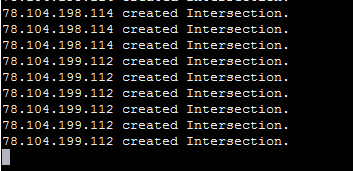
\includegraphics[width=0.65\textwidth]{BilderAllgemein/ampelserver.png}
\end{center}
	\caption{Ausgabe Ampelserver}
	\label{img:ampel}
\end{figure}

\section{Erstellen und Löschen von Hindernisse}

Um im Environment Hindernisse zur Laufzeit zu Erstellen, muss dem Terrain-GameObject ein Skript (Obstacles.cs) hinzugefügt werden. In diesem Skript findet die Abarbeitung des Inputs des Users statt.

Wie bereits in \ref{Hindernisse} erläutert wird zum Start der Verkehrssimulation das Hindernis geladen. Dies erfolgt über den "Load" Befehl.

\begin{lstlisting}[caption={Laden des Hindernisses},label={lst:Hinderniss_laden}]
private GameObject prefabLog;
void Start()
{
	prefabLog = Resources.Load("Rock", typeof(GameObject)) as GameObject;
}
\end{lstlisting}

Der in \ref{Hindernisse} beschrieben soll ein Button gedrückt gehalten werden um Hindernisse spawnen zu können. Dieser wird über einen KeyCode definiert. Im Skript wird nun in jedem Update Aufruf darauf gewartet, ob der definierte Button gedrückt und ein "MouseDown" Event vorkommt. Mit diesem Event kann die Position der Maus auf dem Bildschirm herausgefunden werden, jedoch stimmen diese nicht mit den Welt-Koordinaten überein. Deshalb muss hier eine Umwandlung durchgeführt werden, welche mit Hilfe eines Raycasts gelöst wurde. Durch das Instanzieren wird das neu erstellte Hindernis in der Welt platziert.

\begin{lstlisting}[caption={Erstellen des Hindernisses},label={lst:Hinderniss_erstellen}]
private KeyCode shiftLeft = KeyCode.LeftShift;
if(Input.GetMouseButtonDown(0) && Input.GetKey(shiftLeft)) //Left mouse button clicked
{
	Vector3 mousePosition = Input.mousePosition;
	var ray = Camera.main.ScreenPointToRay(mousePosition);
	RaycastHit hit;
	if(Physics.Raycast(ray, out hit, 1000f))
	{
		Vector3 position = hit.point;			Vector3 yOffset = new Vector3(0, 1.5f, 0);
		position += yOffset;			
		GameObject prefabInstance = Instantiate(prefabLog, position, new Quaternion()) as GameObject;
	}
}
\end{lstlisting}

Zum Löschen eines Hindernisses muss die rechte Maustaste in Kombination mit dem vorher definierten Button verwendet werden. Mittels "Destroy" wird anschließend das erkannte GameObject wieder von der Welt gelöscht.

\begin{lstlisting}[caption={Zerstören des Hindernisses},label={lst:Hinderniss_zerstören}]
if(Input.GetMouseButtonDown(1) && Input.GetKey(shiftLeft)) //Right mouse button clicked
{
	Vector3 mousePosition = Input.mousePosition;
	var ray = Camera.main.ScreenPointToRay(mousePosition);
	RaycastHit hit;
	if(Physics.Raycast(ray, out hit, 1000f))
	{
		Vector3 position = hit.point;
		GameObject collidedObject = hit.collider.gameObject;
		if(collidedObject.name.Equals("Rock(Clone)"))
		{
			Destroy(collidedObject);
		}
	}
}
\end{lstlisting}

\begin{figure}[H]
\begin{center}
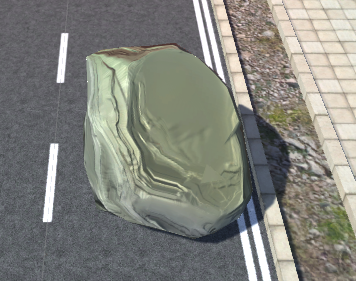
\includegraphics[width=0.5\textwidth]{BilderAllgemein/rock.PNG}
\end{center}
	\caption{Hindernis}
	\label{img:hindernis}
\end{figure}

\section{Aus- und Einfahren von Fahrzeugen anderer Gruppen}
\label{Aus-_und_Einfahren_von_Fahrzeugen_anderer_Gruppen}

Mit dem Plugin `Unity3D.Amqp` (\url{https://github.com/CymaticLabs/Unity3D.Amqp}) für Unity ist es möglich einen RabbitMQ-Server direkt in Unity einzubinden.

Die Konfiguration der Serverdaten werden dabei direkt in den Menüeinstellungen von Unity vorgenommen. Die verwendete Konfiguration ist in Abbildung \ref{img:rabbit} zu sehen.

\begin{figure}[H]
\begin{center}
	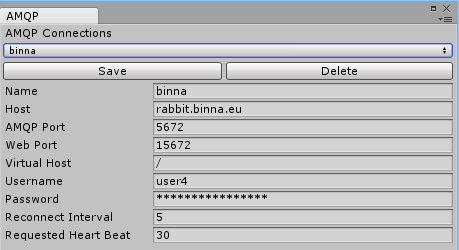
\includegraphics[width=0.9\textwidth]{BilderAllgemein/rabbitconfig.png}
\end{center}

	\caption{Einstellungen RabbitMQ}

	\label{img:rabbit}
\end{figure}

Jede Gruppe bekam einen eigenen Benutzer samt Passwort. Damit man Nachrichten empfangen kann, muss man sich auf eine `Queue` subscriben.

Das Plugin stellt anschließend Methoden zur Verfügung. Eine solche Methode ist \texttt{OnMessageReceived()}. Damit lässt sich eine eingehende Nachricht an ein Objekt in der Spielwelt weitergeben. Das Objekt kann daraufhin reagieren, beispielsweise ein Auto erzeugen.

\begin{figure}[H]
\begin{center}
	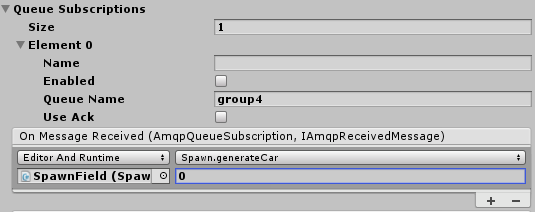
\includegraphics[width=0.9\textwidth]{BilderAllgemein/rabbitqueue.png}
\end{center}

	\caption{RabbitMQ Queue}

	\label{img:rabbitq}
\end{figure}

In Abbildung \ref{img:rabbitq} sieht man wie eine eingehende Nachricht beim Objekt \texttt{SpawnField} eine Methode aufruft.